\documentclass{article}
\title{Efficient Planning for Sokoban with Answer Set Programming - A Case Study}
\author{Thomas Verweyen}
\date{\today}
\usepackage{listings}
\usepackage{graphicx}
\graphicspath{{./images/}}
\usepackage{color}
\lstset{numbers=left,
literate = {-}{-}1,
basicstyle=\footnotesize,
numbersep=5pt, backgroundcolor=\color{white},
captionpos=b,keywordstyle=\color{blue},
commentstyle=\color{green}}
\begin{document}
\maketitle
\renewcommand*\contentsname{Summary}
\tableofcontents
\newpage
\section*{Abstract}
Sokoban approach with ASP planning $\rightarrow$ PlainEnc, IncEnc, Optimization (?)
\section{Introduction}
%%%%TODO: REWORK THIS
What do i do? I'm working on the Sokoban problem and trying to do my best to find a fast and easy solution to it. I'm not working on any level but just the ones meeting some criteria. I'm picking qualitative and quantitative characteristics and deciding on some values to examine. My encodings are supposed to work better on some of the instances and worse on others. What rules describe those fluctuations? What assumptions can be made? Is there a trend when comparing runtimes to my qualitative and quantitative characteristics? E.g. you would expect the runtime to go up when the instance's size grows or when the amount of boxes in the level grows.
In this thesis I will work on optimizing ASP encodings for the game Sokoban towards different instances. First Ill briefly explain what Sokoban is and how it is played, then Ill give a short introduction on comparable/similar/other scientific studies concerning sokoban. Then Ill go over my work, ... and finally evaluation and Discussion of Results.
\newpage
\section{What is Sokoban}
\subsection{Background}
%% ZU KURZ, MIR FEHLT EIN BISSCHEN LORE (SOKOBAN HEISST WARENHAUSMANN, ENTWICKELT VON.., ...) UND EIN BISSCHEN FORMALITÄT (VGL \cite{Froleyks2017UsingAA})
Sokoban is a logistic planning puzzle game from Japan. Sokoban was apparently created by Hiroyuki Imabayashi in 1981, and published by \textit{Thinking Rabbit} in 1982. Sokoban means warehouse person in japanese. The game has very simple rules but shows to be very complex for humans and for AI. This makes Sokoban a very interesting subject for research regarding planning problems.
%LOT OF RESEARCH REGARDING THAT (SO COMPLEX, SO EXEMPLARY, SO RELATABLE TO REAL LIFE AI PROBLEMS, SO EASY TO RESEARCH)
\subsection{Rules}
\begin{figure}[h]
\centering
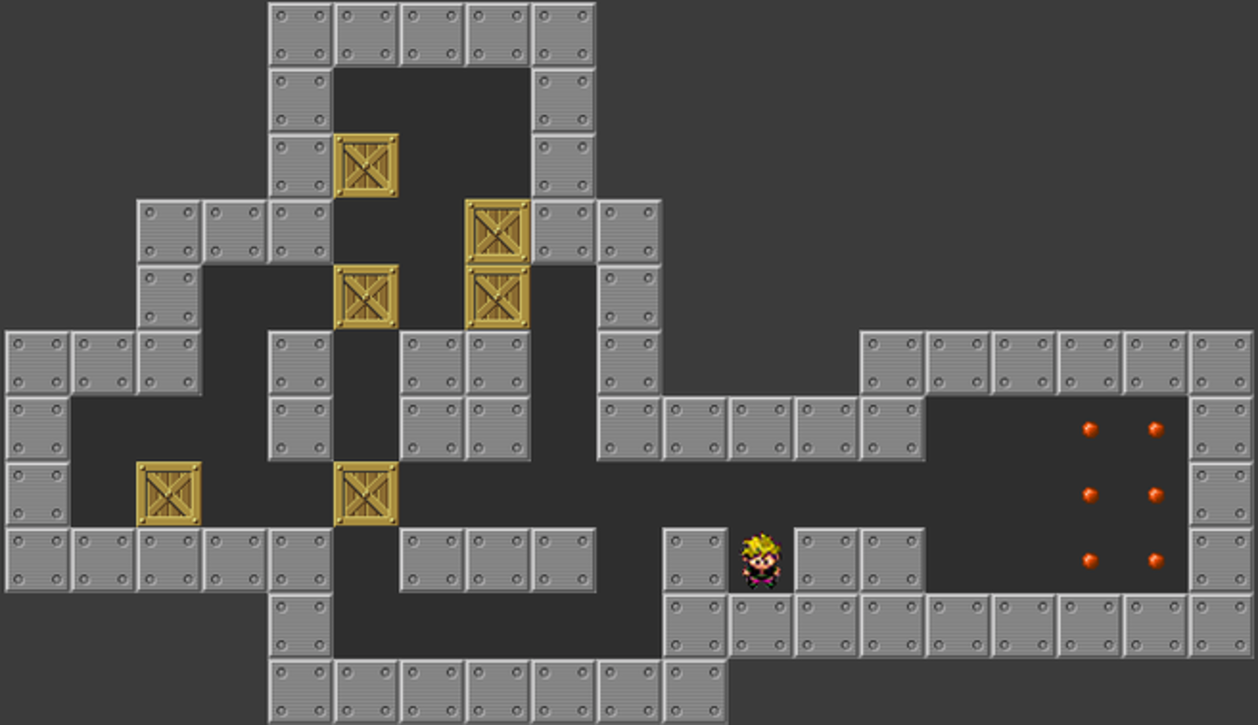
\includegraphics[scale=0.2]{SokobanLevel1}
\caption{First of the Classical Sokoban Levels}
\label{fig:1}
\end{figure}
Figure \ref{fig:1} illustrates the first Sokoban level of the original set of levels. The game is played on a board that can be modelled as a two-dimensional grid. The squares can either be floor or wall squares. Some floor squares are marked as goals and the same number of floor squares contain boxes. The player pushes boxes around this modelled warehouse, trying to cover the marked goal fields (targets) with one of the boxes. For that the player can move one step at a time into one of the four directions \textit{up}, \textit{down}, \textit{left} and \textit{right}. When the player moves onto a box's position the box is pushed one field into the direction of the move. There can never be multiple boxes on one field, neither can there be a box where there is no field. A \textit{solution} to a level is a sequence of moves that leaves a box on each target.
In many of the levels created to this date, the warehouse has a lot of small passageways and very intricate designs. In this thesis I will look at more open level designs, e.g. rectangular levels.
Sokoban is a very difficult planning problem for multiple reasons. There are a lot of possibilities to create a deadlock (a gamestate from which no solution can be found), the branching factor is large and the optimal solution can be very long \cite{BoteaHeuristicsVsPlanning}.

%Sokoban is a logistics game, where the player controls a character in a warehouse. The goal of the game is to move all crates in the warehouse on one of the target fields. The rules state that crates cannot be stacked on one field and crates cannot be pushed if there is a crate or a wall blocking the way. Each player move is a step into one of the four directions in a two-dimensional grid. If the player would collide with a crate, the crate is pushed into the direction of the player-movement. A level is usually satisfied when each crate is pushed on a target; also we can conclude that each target would be covered with a crate, because the amount of targets and crates is equal.
\newpage
\section{State of the Art}
\paragraph*{•}
\textbf{Complexity:} Gordon Wilfong published in 1991 that all motion planning problems with moving obstacles are NP-hard \cite{WilfongNPhard}. He proved this by reducing $3$-$Sat$ to such a problem. The question whether Sokoban is PSPACE-complete remained open until 1997, when Joseph C. Culberson published his paper "Sokoban is PSPACE-complete" \cite{PSpaceComplete}. He found a transformation algorithm to transform an LBA into a level of Sokoban, with the solution to the level having a number of steps in $\Theta (|w|+t(|w|))$, where $w$ is the input and $t(|w|)$ is the amount of transitions the LBA made. %This shows PSPACE-hardness and Sokoban is known to be in PSPACE, so Sokoban is PSPACE-complete.
%He didnt answer the question whether Sokoban is also PSPACE-complete. That was answered by Joseph C Culberson \cite{PSpaceComplete} in 1997. He showed that it is possible to emulate a linear bounded automaton by constructing a level. The solution to this constructed level, if there is any, will have a length in $\Theta (|w|+t(|w|))$, where $w$ is the input and $t(|w|)$ is the amount of transitions the LBA made. This shows PSPACE-completeness
\paragraph*{•}
\textbf{Approaches:} There are loads of different researches regarding approaches to Sokoban. I decided which to show. Botea et al. found out that heuristics, while significantly improving chess AI, do not seem to help for planning the soko puzzle \cite{BoteaHeuristicsVsPlanning}. Planning would be a better approach. So to get there and create good plans like humans would, the solver will start meta-reasoning by recognizing rooms and tunnels. Then using those rooms and tunnels to create a plan where first a way is found to bring the crates from the room where theyre at to the target room. Then another plan is made to organize crates in a room.
\paragraph*{•}
\textbf{Macromoves:} Macromoves are a planning strategy that is so successful it is implemented in several good Sokoban solvers. The best example would be Rolling Stone, an excellent Sokoban solver, with a lot of optimizations implemented. One of the optimizations is the possibility to create macromoves for tunnels to reduce all states in the tunnel to one or two, reducing the search space severely.
\paragraph*{•}
\begin{figure}[h]
\centering
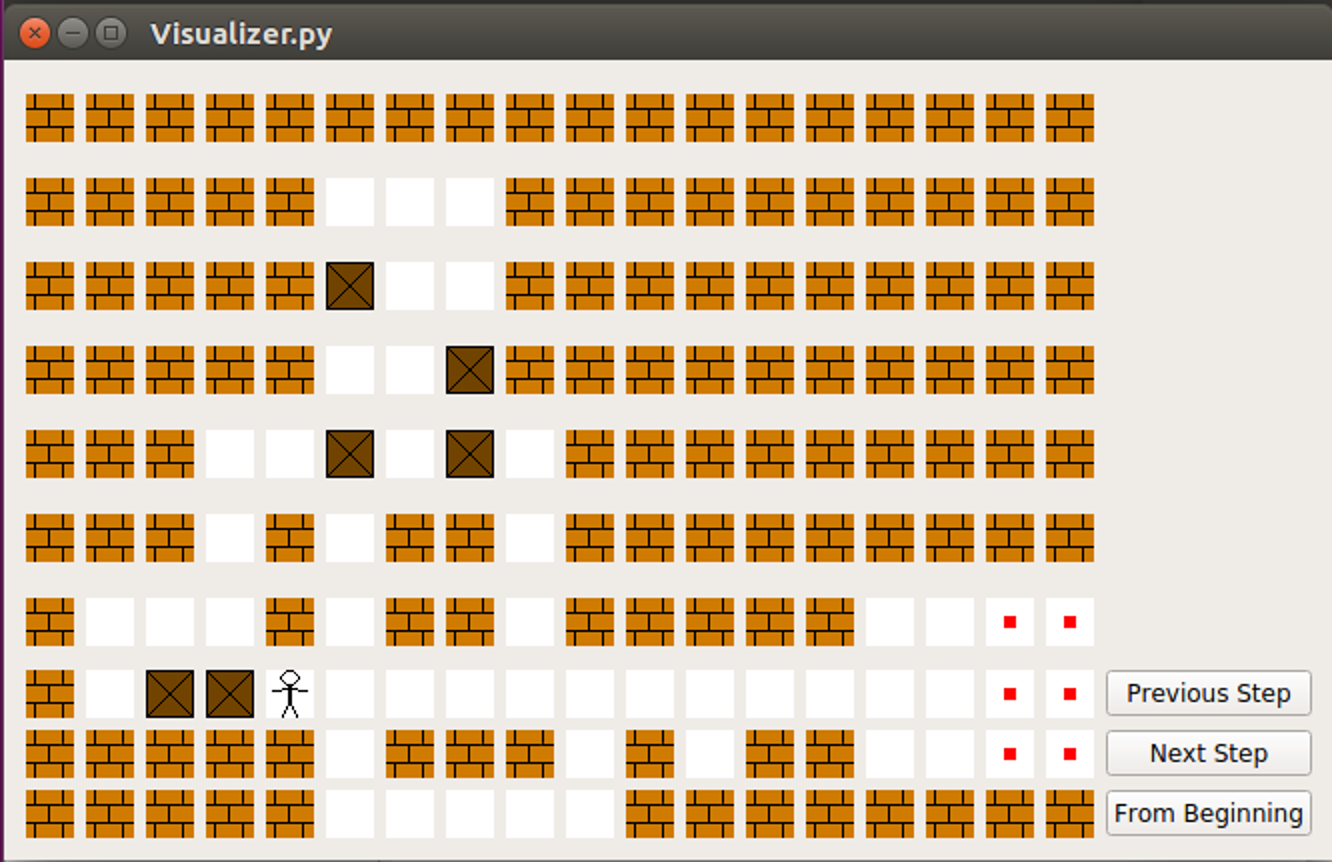
\includegraphics[scale=0.2]{flipped,deadlockexample}
\caption{Deadlock example}
\label{fig:2}
\end{figure}
\begin{figure}[h]
\centering
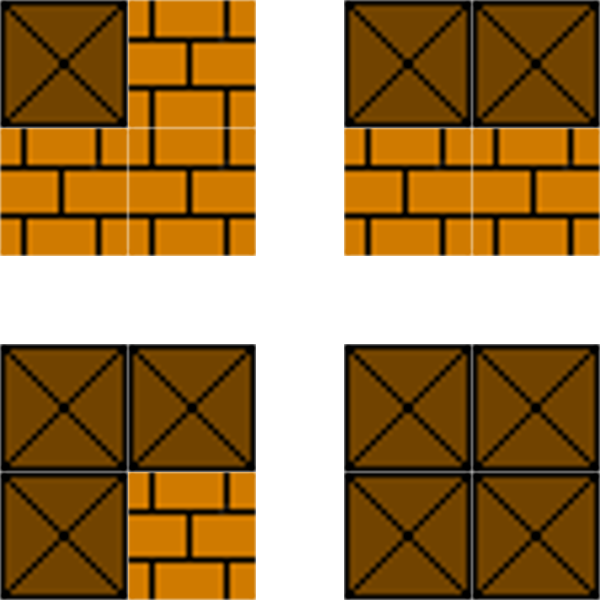
\includegraphics[scale=0.2]{deadlocktypes}
\caption{Deadlock types}
\label{fig:3}
\end{figure}
\textbf{Deadlock Detection:} Deadlocks are states from which no solution can be found. A trivial example for a deadlock (see Figure \ref{fig:2}) is a box pushed into a corner with no target under it. The box cannot be pulled, so it cannot be recovered from the corner, but to find a solution all boxes have to be covering a target.
Detecting deadlocks the moment they appear is a very powerful optimization, for the reason that huge parts of the search tree can be eliminated early on, without further looking into them. The problem with this strategy is that deadlocks can be very hard to detect, e.g. when they consist of multiple boxes blocking each other in some kind of tunnelsystem. Deadlocks are easier to detect and remove from the search tree when the domain is restricted. When looking at levels with a rectangular shape there are four common deadlocks, cp. Fig. \ref{fig:3}.
\paragraph*{•}
%% A: Box in Corner, B: Doublebox on wall, C: Three boxes on corner, D: Four boxes building a square
%What is a Deadlock, with picture. Why do you detect those? How do you detect those? Better when you know the level or know basic deadlocks to look for. In the halls without tunnels it should be less hard
\textbf{Relevance Cutting:} A basic AI to solve a planning problem like Sokoban will look at all possible ways to move around the level, but some of those are dubious but legal or just plain irrelevant. In a lot of cases those dubious ways do not lead to an optimal solution, but of course a problem can be constructed where the optimal solution can only be found when looking at those dubious cases. So Junghanns and Schaeffer tried to teach their AI meta-reasoning to give it the ability to know when to look at those dubious ways and when to ignore them. This they did by creating an influence measurement and only taking moves that are influenced by prior moves, to prevent actions that are disembodied from all prior moves (and seem irrelevant).
%Relevance Cutting tries to remove the problem of really stupid AI moves, like lrlrlrlrlrlrlr, by trying to teach the AI to know relevance, by teaching it influence of one move over another. This means that the moves can't be without any connection to each other and that the AI can realize that two parts of the puzzle have no influence on each other implying that order between the parts doesnt matter. the approach is statistic not dynamic which makes it rather simple and improvable.
%Heuristics doesnt seem to do a great deal for sokoban \cite{BoteaHeuristicsVsPlanning}. It helped a lot with chess e.g., but doesnt cut it for sokoban. Approach the hard domain of sokoban in another way. Macromoves a way that really works well and is used in practice, also deadlock detection (WHAT IS A DEADLOCK - stone in corner and no goal -> no solutions) (obviously best if you know the specific level). Reference Rolling stone (source not available (?)). Furthermore Sokoban can be abstracted into rooms and tunnels, making it into subproblems which should be easier to solve, tunnels for example, are mostly immediately solved. Similarly you can also use relevance cutting. This means creating a measurement for relevance in between moves and picking moves that are relevant to prior moves (few exceptions in special cases).Backwards Approach and LexOrdering.Conclusion
%Sokoban was researched to be PSPACE-complete and NP-hard. PSPACE-complete was done by constructing levels that are PSPACE-complete (look at the work again!!). Heuristic seems to be of little use, so go for planning instead [botea]
%Sokoban can be abstracted into subproblems to get more smaller problems, greatly reducing searchspace.
%This also makes sense in relevance cutting, which looks at relations between boxes to find groups that behave together and cleanly separate those.
%Alternatively Backwards Approach
%Or LexOrdering
%All in all a Plethora of different approaches to crack the problems of sokoban.
%- mention other works on Sokoban
%- what tests?
%- what results?
%- whats the connection?
\newpage
\section{My Work}
\paragraph*{•}
In 
what did i do?
what is my baseline?
what changes from encoding to encoding
which of the encodings works best in which kind of instance
how do i evaluate that
show my experiments and their results
\subsection{Encodings}
\subsubsection{Fact Format}
\paragraph*{•}
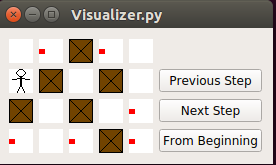
\includegraphics{Visualizer}
\lstinputlisting{../InstancesClean/Inst-A-Z20-6Halle.lp}
\subsubsection{Plain Encoding}
\paragraph*{•}
\lstinputlisting{../Encodings/SokobanPlainEncoding.lp}
The first try to construct a naive encoding to solve sokoban-instances yielded a solution that works in a common way in ASP planning. In line 4 we initialize the information from the level instance with the time 0. In line 7 we state that there is one move at minimum and at maximum for each timestep. This makes the ASP planner ground all sequences of moves, pick one for every timestep and infer every successive state from the moves it picks. In lines 9-13 we calculate the successor state from the move picked in line 7. Line 9 calculates the new player-position, line 11 calculates the new position of the box in the players way and line 13 calculates the new position of boxes not touched by the player. Additionally we need some integrity constraints to prevent illegal states. The integrity constraint in line 15 ensures that at no time a box or player has a position outside of the playing field. The integrity constraint in line 17 ensures that at no time boxes or the player share one field.
In the lines 19-21 we define our win-condition to be that all targets in the instance have to be covered by boxes.
The Plain Encoding has the predicates, time/1, dir/2, at/4, move/3, uncovered/3, goal/3
The encoding works in a common way in ASP planning, by guessing the sequence of actions and inferring the successor states by effect axioms. There is a time/1 predicate for every timestep and a at/4 predicate for every box and the player at every timestep.

\subsubsection{Incremental Encoding}
\paragraph*{•}
\lstinputlisting{../Encodings/SokobanPlainEncodingInc.lp}
The incremental encoding is similar to the plain encoding. The difference is the partition of the encoding into three parts: the \#program base in lines 3-5 which is independent of the step parameter t, the \#program step in lines 7-19 which is the cumulative part, collecting knowledge and the \#program check in lines 21-25 which is specific for each value of t (STEP ALSO IS THOUGH). This allows for gradually processing each time step and accumulating knowledge that persists even if the current step is not satisfiable.

\subsubsection{Advanced Encoding}
\paragraph*{•}
\lstinputlisting{../Encodings/SokobanPlainEncodingOpti.lp}
\subsection{Evaluation}
\paragraph*{•}
\subsection{Experiments and Results}
\paragraph*{•}
\newpage
\section{Discussion of Results}
\paragraph*{•}
compare chapter State of the Art with chapter My Work \cite{LifschitzASP}

\begin{thebibliography}{}
\bibitem{LifschitzASP}
Vladimir Lifschitz,
\textit{Answer Set Planning},
ICLP, 1999.

\bibitem{Lifschitz2002AnswerSP}
Vladimir Lifschitz,
\textit{Answer set programming and plan generation},
Artificial Intelligence, 2002, Vol. 138, p.39-54.

\bibitem{LifschitzWhatisASP}
Vladimir Lifschitz,
\textit{What is Answer Set Programming?},
AAAI, 2008.

\bibitem{Gebser2013RicochetRA}
Martin Gebser, Holger Jost, Roland Kaminski, Philipp Obermeier, Orkunt Sabuncu, Torsten Schaub, Marius Thomas Lindauer,
\textit{Ricochet Robots: A Transverse ASP Benchmark},
LPMNR, 2013.

\bibitem{BoteaHeuristicsVsPlanning}
Adi Botea, Martin Müller, Jonathan Schaeffer,
\textit{Using Abstraction for Planning in Sokoban},
Computers and Games, 2002.

\bibitem{Frisch2006PropagationAF}
Alan M. Frisch, Brahim Hnich, Zeynep Kiziltan, Ian Miguel, Toby Walsh,
\textit{Propagation algorithms for lexicographic ordering constraints},
Artificial Intelligence, 2006, Vol. 170, p.803-834.

\bibitem{Dor1999SOKOBANAO}
Dorit Dor, Uri Zwick,
\textit{SOKOBAN and other motion planning problems},
Computational Geometry, 1999, Vol. 13, p.215-228.

\bibitem{Froleyks2017UsingAA}
Nils Christian Froleyks and Tom{\'a}{\^s} Balyo,
\textit{Using an Algorithm Portfolio to Solve Sokoban},
SOCS, 2017.

\bibitem{PSpaceComplete}
Joseph C. Culberson,
\textit{Sokoban is PSPACE-complete},
1997.

\bibitem{SokoRelevanceCuts}
Andreas Junghanns, Jonathan Schaeffer,
\textit{Sokoban: Improving the Search with Relevance Cuts},
Journal of Theoretical Computing Science, 1999, Vol. 252, p.1-2.

\bibitem{SymmetryBreaking}
Brahim Hnich, Zeynep Kiziltan, Toby Walsh,
\textit{Combining Symmetry Breaking with Other Constraints: Lexicographic Ordering with Sums},
ISAIM, 2004.

\bibitem{WilfongNPhard}
Gordon Wilfong,
\textit{Motion planning in the presence of movable obstacles},
Annals of Mathematics and Artificial Intelligence, 1991.
\end{thebibliography}


\end{document}